% ============================================================================
%  PRL Article: Modeling Two-Dimensional Supersonic Marshak Waves
%  Uses revtex4-2 (APS journal style)
% ============================================================================
\documentclass[prl, twocolumn, superscriptaddress, amsmath, amssymb, reprint]{revtex4-2}

\usepackage{graphicx}
\usepackage{amsmath}
\usepackage{amssymb}
\usepackage{bm}
\usepackage{hyperref}
\usepackage{xcolor}
\usepackage{microtype}

\graphicspath{{figures/}}

\begin{document}

% ----------------------------------------------------------------------------
%  Title
% ----------------------------------------------------------------------------
\title{Semi-Analytic Two-Dimensional Model for Supersonic Marshak Waves in Cylindrical Geometry}

\author{Yuval Kochavi}
\affiliation{Racah Institute of Physics, The Hebrew University of Jerusalem, Jerusalem 91904, Israel}

\author{Tal Ramot}
\affiliation{Racah Institute of Physics, The Hebrew University of Jerusalem, Jerusalem 91904, Israel}

\author{Tal Balakirski}
\affiliation{Racah Institute of Physics, The Hebrew University of Jerusalem, Jerusalem 91904, Israel}

\author{Shay I.~Heizler}
\affiliation{Racah Institute of Physics, The Hebrew University of Jerusalem, Jerusalem 91904, Israel}

\date{\today}

% ----------------------------------------------------------------------------
%  Abstract
\begin{abstract}
We present a semi-analytic model for radiation-wave propagation in finite cylindrical foam targets that combines a self-consistent radiative boundary condition and global energy balance with the leading effects of wall interaction and hydrodynamic response. The model predicts the longitudinal heat-front evolution and its transverse curvature, using experiment-specific drive histories and material properties. Comparisons with representative experiments and two-dimensional diffusion simulations show that the framework captures the main trends in front propagation, breakout, curvature, and sleeve dependence. The model therefore provides a compact and physically transparent description of finite-target radiative transport in the diffusive regime.
\end{abstract}

\maketitle

% ============================================================================
%  I. INTRODUCTION
% ============================================================================
% \section{Introduction}
\begingroup
\setlength{\parskip}{0pt}
\setlength{\parindent}{1em}
Radiative heat waves are central to inertial-confinement fusion (ICF) and high-energy-density physics~\cite{AbuShawareb2024,AbuShawareb2022}. In indirect-drive ICF, laser energy is converted into x~rays within a high-$Z$ hohlraum, whose radiation heats and compresses the fusion capsule~\cite{Lindl2004}. A first-principles description must couple nonlinear laser propagation, opacities, equations of state, hydrodynamics and many more. Because a unified treatment remains impractical, individual physical processes must be isolated and studied independently. Here, we focus on dedicated experiments designed to probe radiation transport under controlled conditions.

Early experiments by Afshar-rad \textit{et al.} and Massen \textit{et al.} established low-density foams as a controlled platform in which radiation-driven fronts could outrun the hydrodynamic response~\cite{AfsharRad1994,Massen1994}. Back \textit{et al.} then reported the first detailed measurements of a diffusive, supersonic radiation wave in a finite cylindrical foam several optical depths thick~\cite{Back2000PRL}. They observed a curved front that broke out first on axis and later near the wall, directly exposing the role of energy loss to the surrounding sleeve. A companion study broadened the analysis across materials, optical depths, and target lengths~\cite{Back2000POP}, and subsequent experiments have explored diverse foams, sleeves, drives, and geometries~\cite{Jiang2005,Keiter2008,Zhang2010,Moore2015,Courtois2024}.

Theory, however, remains fragmented. The one-dimensional Hammer--Rosen diffusion solution describes on-axis propagation~\cite{Hammer2003}, and later extensions include wall-energy loss, ablation, compression, and boundary-temperature corrections to get quantitative agreement with the experimental data~\cite{Cohen2018,Cohen2020Key}. These models do not capture the measured delay between front arrival on axis and at the tube boundary. Conversely, curvature models describe front bending~\cite{Hurricane2006,Courtois2022}, but represent wall coupling by a fitted constant and do not accurately reproduce the on-axis evolution.

In this work, we present a semi analytic two-dimensional model that self-consistently connects longitudinal propagation and radial curvature in finite cylindrical foams. The framework combines a corrected Hammer--Rosen solution for the radiative boundary, wall losses, hydrodynamic effects, and finite-size transport with cylindrical eigenmodes whose transverse structure is set by a time-dependent wall albedo~\cite{Hurricane2006,Courtois2022}. By capturing both the front evolution and its geometry within one physically transparent description, the model enables systematic interpretation of experiments across different target dimensions, foam properties, and sleeve materials, and provides a practical tool for identifying the mechanisms that control radiative transport.

Figure~\ref{fig:setup_tdrive} illustrates the generic experimental platform: the cylindrical foam-tube target~(a) and a representative hohlraum drive history~(b)~\cite{Back2000PRL}.
\endgroup

\begin{figure}[ht]
    \centering
    \begin{minipage}{0.5\columnwidth}
        \centering
        
\includegraphics[width=\linewidth]{figures/setup.png}
        \vspace{-0.5em}
        \centerline{(a)}
    \end{minipage}\hfill
    \begin{minipage}{0.5\columnwidth}
        \centering
        
\includegraphics[width=\linewidth]{figures/T_drive.png}
        \vspace{-0.5em}
        \centerline{(b)}
    \end{minipage}
    \caption{(a) Experimental platform: laser beams enter the hohlraum through the LEH, generate x rays, and drive a Marshak wave in low-density foam targets of different lengths~\cite{Moore2015}. (b) Measured hohlraum drive temperature $T_D(t)$ for the high-energy Back experiment~\cite{Back2000PRL}.}
    \label{fig:setup_tdrive}
\end{figure}


% ============================================================================
%  II. MODEL
% ============================================================================

In the supersonic regime the hydrodynamic response is slow compared with the radiative front, so matter remains nearly stationary during propagation. Under the additional assumptions of LTE and diffusive transport---valid when the foam is several optical depths thick---radiation and matter share a single temperature $T(x,r,t)$, and the coupled system reduces to a nonlinear diffusion equation~\cite{Pomraning1979,Rosen2009}:
\begin{equation}\label{eq:diffusion}
\frac{\partial (aT^4)}{\partial t} + \rho\frac{\partial e}{\partial t}
= \nabla\!\cdot\!\left(\frac{c}{3\kappa \rho}\nabla\left(aT^4\right)\right),
\end{equation}
where $e$ is the specific internal energy, $\kappa$ the Rosseland mean opacity, $a$ the radiation constant, and $c$ the speed of light. Because both $e$ and $\kappa$ depend on temperature, the problem is strongly nonlinear. We model Eq.~\eqref{eq:diffusion} in two stages. First, we compute a corrected one-dimensional longitudinal evolution that includes (i)~a self-consistent surface flux, (ii)~wall-energy losses, (iii)~wall ablation and foam compression~\cite{Cohen2020Key,Cohen2018}, and (iv)~finite-diameter transport corrections~\cite{Courtois2024}. Second, we reconstruct the time-dependent two-dimensional front curvature from sleeve-coupled absorption~\cite{Hurricane2006,Courtois2022}.

For the first stage, the one-dimensional Hammer--Rosen framework~\cite{Hammer2003,Rosen2009} assumes power-law forms for opacity and material energy,
$\frac{1}{\kappa}=gT^{\alpha}\rho^{-\lambda}$ and $e=fT^{\beta}\rho^{-\mu}$. Using perturbation theory for the 1D version of the diffusion equation~\eqref{eq:diffusion}, the heat-front position is given by
\begin{equation}\label{eq:HR}
    x_F^2(t) = \frac{2+\varepsilon}{1-\varepsilon}\,C\,H^{-\varepsilon}(t)\int_0^t H(t')\,dt',
\end{equation}
where $H(t) = T_s^{4+\alpha}(t)$, $\varepsilon = \beta/(4+\alpha)$, and
	$C = \frac{16\,g\,\sigma_{\mathrm{SB}}}{3f(4+\alpha)}\,\rho^{2-\mu-\lambda}$.
For each material, the opacity and EOS exponents and coefficients ($\alpha,\beta,\lambda,\mu,g,f$) are not newly fitted in this work. We adopt the tabulated values reported by Cohen \textit{et al.}~\cite{Cohen2020Key}, where the parameters were fitted in the relevant experimental regime using SESAME and exact-opacity CRSTA tables, with QEOS tables for heat capacity. Therefore, differences between experiments arise primarily from material-property differences together with the experiment-specific drive temperature reported in the corresponding references~\cite{Back2000PRL,Back2000POP,Moore2015,Courtois2024}.

Because the HR front evolution takes $T_s(t)$ as an input, it is essential to distinguish between the drive temperature $T_D(t)$ and the foam surface temperature $T_s(t)$. The naive choice $T_s(t)=T_D(t)$ gives an incorrect front evolution and systematically overpredicts the propagation speed. In our reference $\mathrm{SiO}_2$ low-energy case~\cite{Back2000PRL}, this uncorrected HR closure overestimates the front position by about a factor of 1.5 (Fig.~\ref{fig:sio2_low_energy}).

To determine the surface temperature $T_s(t)$, we couple the Marshak boundary condition~\cite{Pomraning1979,Olson2000}, $\sigma_{\mathrm{SB}}T_D^4=\sigma_{\mathrm{SB}}T_s^4+\tfrac{1}{2}F(0,t)$, with the HR boundary energy balance $\dot{E}(t)=F(0,t)$. This closes $T_s(t)$ through the boundary flux instead of setting $T_s=T_D$, yields a physically constrained temperature history for the front solution, and avoids ad hoc temperature-reduction factors. implementation details are given in the SM (see also Ref.~\cite{Cohen2018}).

We now extend the model to 2D effects. A primary source of front retardation in cylindrical-tube experiments is radiative energy loss into the surrounding walls. As the heat wave propagates along the axis, each axial slice of foam is exposed to radiation starting at its local front-arrival time, and the wall at that position absorbs energy over the remaining evolution time. The cumulative wall-loss term is evaluated with the cylindrical integral formulation and material-dependent self-similar wall-heating laws described in the SM~\cite{Shussman2015,Cohen2020Key,Cohen2018}.
Wall losses reduce the energy retained by the foam and therefore slow the front (Fig.~\ref{fig:sio2_low_energy}).

Beyond direct energy removal, the heated wall ablates inward, reducing the effective tube radius over time. This ablation effect is relevant only for high-$Z$ and mid-$Z$ sleeve materials, which are subsonic in the relevant temperatures~\cite{ZeldovichRaizer2002,PakulaSigel1985,Shussman2015} --- in our experiments, gold and copper. For these cases we use the self-similar subsonic ablation-velocity closure described in the SM~\cite{Cohen2020Key,Shussman2015}, including its density-dependent prefactor calibration for a confined sleeve--foam interface.
In addition, the ablated material compresses the foam, raising the mean density $\rho(t) = \rho_0 V_0 / V(t)$. This retards the front further, making the HR coefficient time dependent through a density-history integral~\cite{Cohen2020Key,Shussman2015}, as described in the SM. Together, wall-energy loss and ablation-driven compression are the dominant 2D corrections that bring the model into quantitative agreement with experiment (Fig.~\ref{fig:sio2_low_energy}).

A further correction is required when the Rosseland mean free path, $\lambda_R = 1/(\kappa\rho)$, becomes comparable to or larger than the tube diameter $2R$. In this regime, transport is no longer dominated solely by absorption and emission. Wall collisions increasingly limit photon propagation and reduce the effective transport length. Following Ref.~\cite{Courtois2024}, we replace $\lambda_R$ with
 $\lambda_{\mathrm{eff}} = \left[\left(2R\right)^{-n} + \lambda_R^{-n}\right]^{-1/n}$,
where $n$ controls the sharpness of the crossover. In the diffusion limit (e.g., the SiO$_2$ low-energy case~\cite{Back2000PRL}, $\lambda_R \ll 2R$), $\lambda_{\mathrm{eff}} \to \lambda_R$, so the correction is negligible. In the wall-collision limit ($\lambda_R \ge 2R$), $\lambda_{\mathrm{eff}} \approx 2R$. The correction is therefore most important in optically thin, low-density foams, where large $\lambda_R$ makes the tube diameter the transport bottleneck and lowers the effective diffusivity below the bulk Rosseland value. In the model, this enters through the time-dependent $\lambda_{\mathrm{eff}}(t)$, which modifies the HR coefficient,
$C(t) = \frac{16\,g\,\sigma_{\mathrm{SB}}}{3f(4+\alpha)t}\,\rho^{2-\mu-\lambda}\,\int_{0}^{t}\lambda_{\mathrm{eff}}(t')dt'$,
and thus the front evolution.

\begin{figure}[h!]
	\centering
	
\includegraphics[width=\columnwidth]{figures/SiO2_low_energy.png}
	\caption{Front-position comparison for the $\mathrm{SiO}_2$ low-energy case, illustrating the effect of the corrected 1D and 2D terms.}
	\label{fig:sio2_low_energy}
\end{figure}

Beyond its agreement with the measured trajectory, Fig.~\ref{fig:sio2_low_energy} shows how the model can separate the relative influence of the physical mechanisms governing the on-axis longitudinal front position. Each curve adds one correction to the preceding model, so the change between successive curves indicates how strongly that effect modifies the front evolution in this experimental configuration. For the $\mathrm{SiO}_2$ low density Ecperimental setup~\cite{Back2000PRL}, the finite MFP correction and direct wall-energy loss produce only small changes, whereas the wall-ablation correction substantially alter the propagation trend. The particularly strong ablation effect follows from the extremely low foam density, $10\,[\mathrm{mg/\,cm^{3}}]$: the density-dependent prefactor calibration approaches unity, allowing greater inward wall motion and stronger foam compression, which increases the mean density and slows the front. This hierarchy is not universal. In other configurations, such as the $\mathrm{SiO}_2$ experiment reported by Back \textit{et al.}~\cite{Back2000POP}, direct wall loss is the dominant correction. The model therefore provides not only a prediction of the front trajectory but also a diagnostic of which mechanism limits propagation in a given target. This information can guide experimental design by identifying whether changes to the drive, foam density, tube diameter, or sleeve material are most likely to increase the front velocity.

While the longitudinal model captures the axial physics and identifies the dominant loss mechanisms, the physical heat front is not planar: radiative losses to the surrounding sleeve cool the tube edge relative to the axis, curving the front and delaying breakout at $r>0$. This curvature is experimentally important because the measured signal is the re-emission intensity, $\Phi\propto T^4$, which strongly amplifies transverse temperature variations~\cite{Back2000POP,Back2000PRL}. As a result, the intrinsically 2D front shape both delays breakout at the diagnostic plane and feeds back on the energy balance, since wall losses are controlled by the boundary-front evolution at $r=R$.

To describe this curvature quantitatively, Hurricane and Hammer~\cite{Hurricane2006} showed that, in the idealized limit of constant opacity, negligible material-energy storage, and a steep heat front, the region behind the front is governed by a Laplace problem. In this formulation, the lossy wall enters through a Robin boundary condition set by the wall albedo (see the SM): only a fraction $\alpha$ of the incident radiative flux is returned to the foam, while $1-\alpha$ is absorbed by the surrounding wall. This partial return cools the tube edge relative to the axis, so the transverse eigenmodes bend the front. For a planar channel these modes are cosines, while in an axisymmetric cylindrical tube the regular radial modes are zeroth-order Bessel modes $J_0$ by symmetry at $r=0$. The cylindrical analogue therefore has the leading-order form~\cite{Courtois2022}
\begin{equation}\label{eq:HH_cyl}
    x_F(r,t) = \frac{1}{\kappa_0}\cosh^{-1}\!\left(1 + \frac{D\kappa_0^2 t}{2}\right)J_0(\kappa_0 r) + \text{H.O.T.}
\end{equation}
The transverse wavenumber is fixed by the wall-loss boundary condition. In the weak-loss, high-albedo limit, $\kappa_0 \approx \sqrt{2\varepsilon}/R$ with $\varepsilon = \tfrac{3}{4}\rho\kappa R(1-\alpha)$ and $\alpha$ the wall albedo. This approximation is accurate for small $\varepsilon$, i.e., $\alpha\to1$. However, for lower-albedo cases, such as copper with $\alpha\sim0.5$ and beryllium with $\alpha\sim0.3$, the small-$\varepsilon$ expansion is no longer sufficient. We therefore compute $\kappa_0$ from a numerical solution of the full transverse eigenvalue problem with the wall-loss boundary condition (see the SM). In this way, $J_0(\kappa_0 r)$ captures the curvature the front.

The key quantity controlling the curvature is the wall albedo. Rather than prescribing a constant fitted value~\cite{Hurricane2006,Courtois2022}, we compute a time-dependent $\alpha(t)=F_{\mathrm{out}}/F_{\mathrm{in}}$ from the local interface energy balance between the incoming radiative flux, the re-emitted flux, and the absorbed wall energy; the explicit expression is given in the SM.
This yields $\varepsilon(t)=\tfrac{3}{4}\rho\kappa R\,[1-\alpha(t)]$ and therefore a time-dependent $\kappa_0(t)$ and front curvature. Stronger wall absorption lowers the albedo, increases $\kappa_0(t)$, and produces a more strongly curved front. In the high-albedo limit $\alpha\to1$, $\kappa_0\to0$, and the model recovers the one-dimensional limit. Thus gold sleeves produce an almost flat front, whereas beryllium sleeves produce a more pronounced curvature.
Opacity also evolves in time through $T(t)$ and directly affects the curvature. This dependence is already included through the power-law closure $\kappa^{-1}=gT^{\alpha}\rho^{-\lambda}$ used in the model.

With this dynamic-albedo closure, we keep the separation of variables form only for the transverse structure and replace the longitudinal factor in Eq.~(\ref{eq:HH_cyl}) by the corrected centerline evolution from the longitudinal model. The resulting front is $x_F(r,t)=x_F(t)J_0\!\left(\kappa_0(t) r\right)$. To validate this approach, we compare the model with 2D diffusion simulations without hydrodynamics (see the SM for simulation details). Figure~\ref{fig:simulation_comparison}(a) shows that the time-dependent curvature driven by the time-dependent albedo agrees well with the simulations at multiple times. The same comparison also shows good agreement between the longitudinal front positions of the model and simulation for the Back \,\textit{et al.}\, experimental configuration. Figure~\ref{fig:simulation_comparison}(b) shows the effect of sleeve material: gold gives the flattest front, copper (with slightly lower average albedo) gives a more curved front, beryllium is more curved still, and vacuum gives the most strongly curved front.

\begin{figure}[t]
    \centering
    \begin{minipage}{0.38\columnwidth}
        \centering
        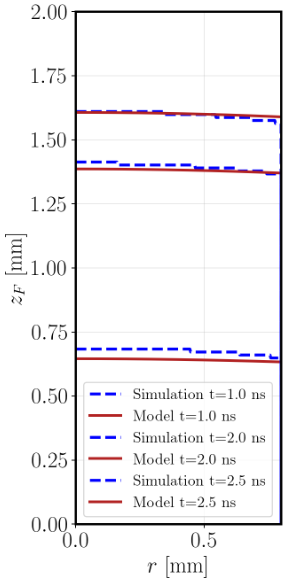
\includegraphics[width=\linewidth]{figures/gold_heyney2.png}
        \vspace{-0.8em}
        \centerline{(a)}
    \end{minipage}\hfill
    \begin{minipage}{0.38\columnwidth}
        \centering
        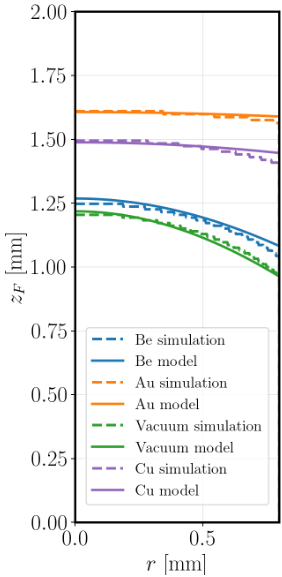
\includegraphics[width=\linewidth]{figures/heyney2.png}
        \vspace{-0.8em}
        \centerline{(b)}
    \end{minipage}

    \vspace{0.4em}
    \begin{minipage}{0.4\columnwidth}
        \centering
        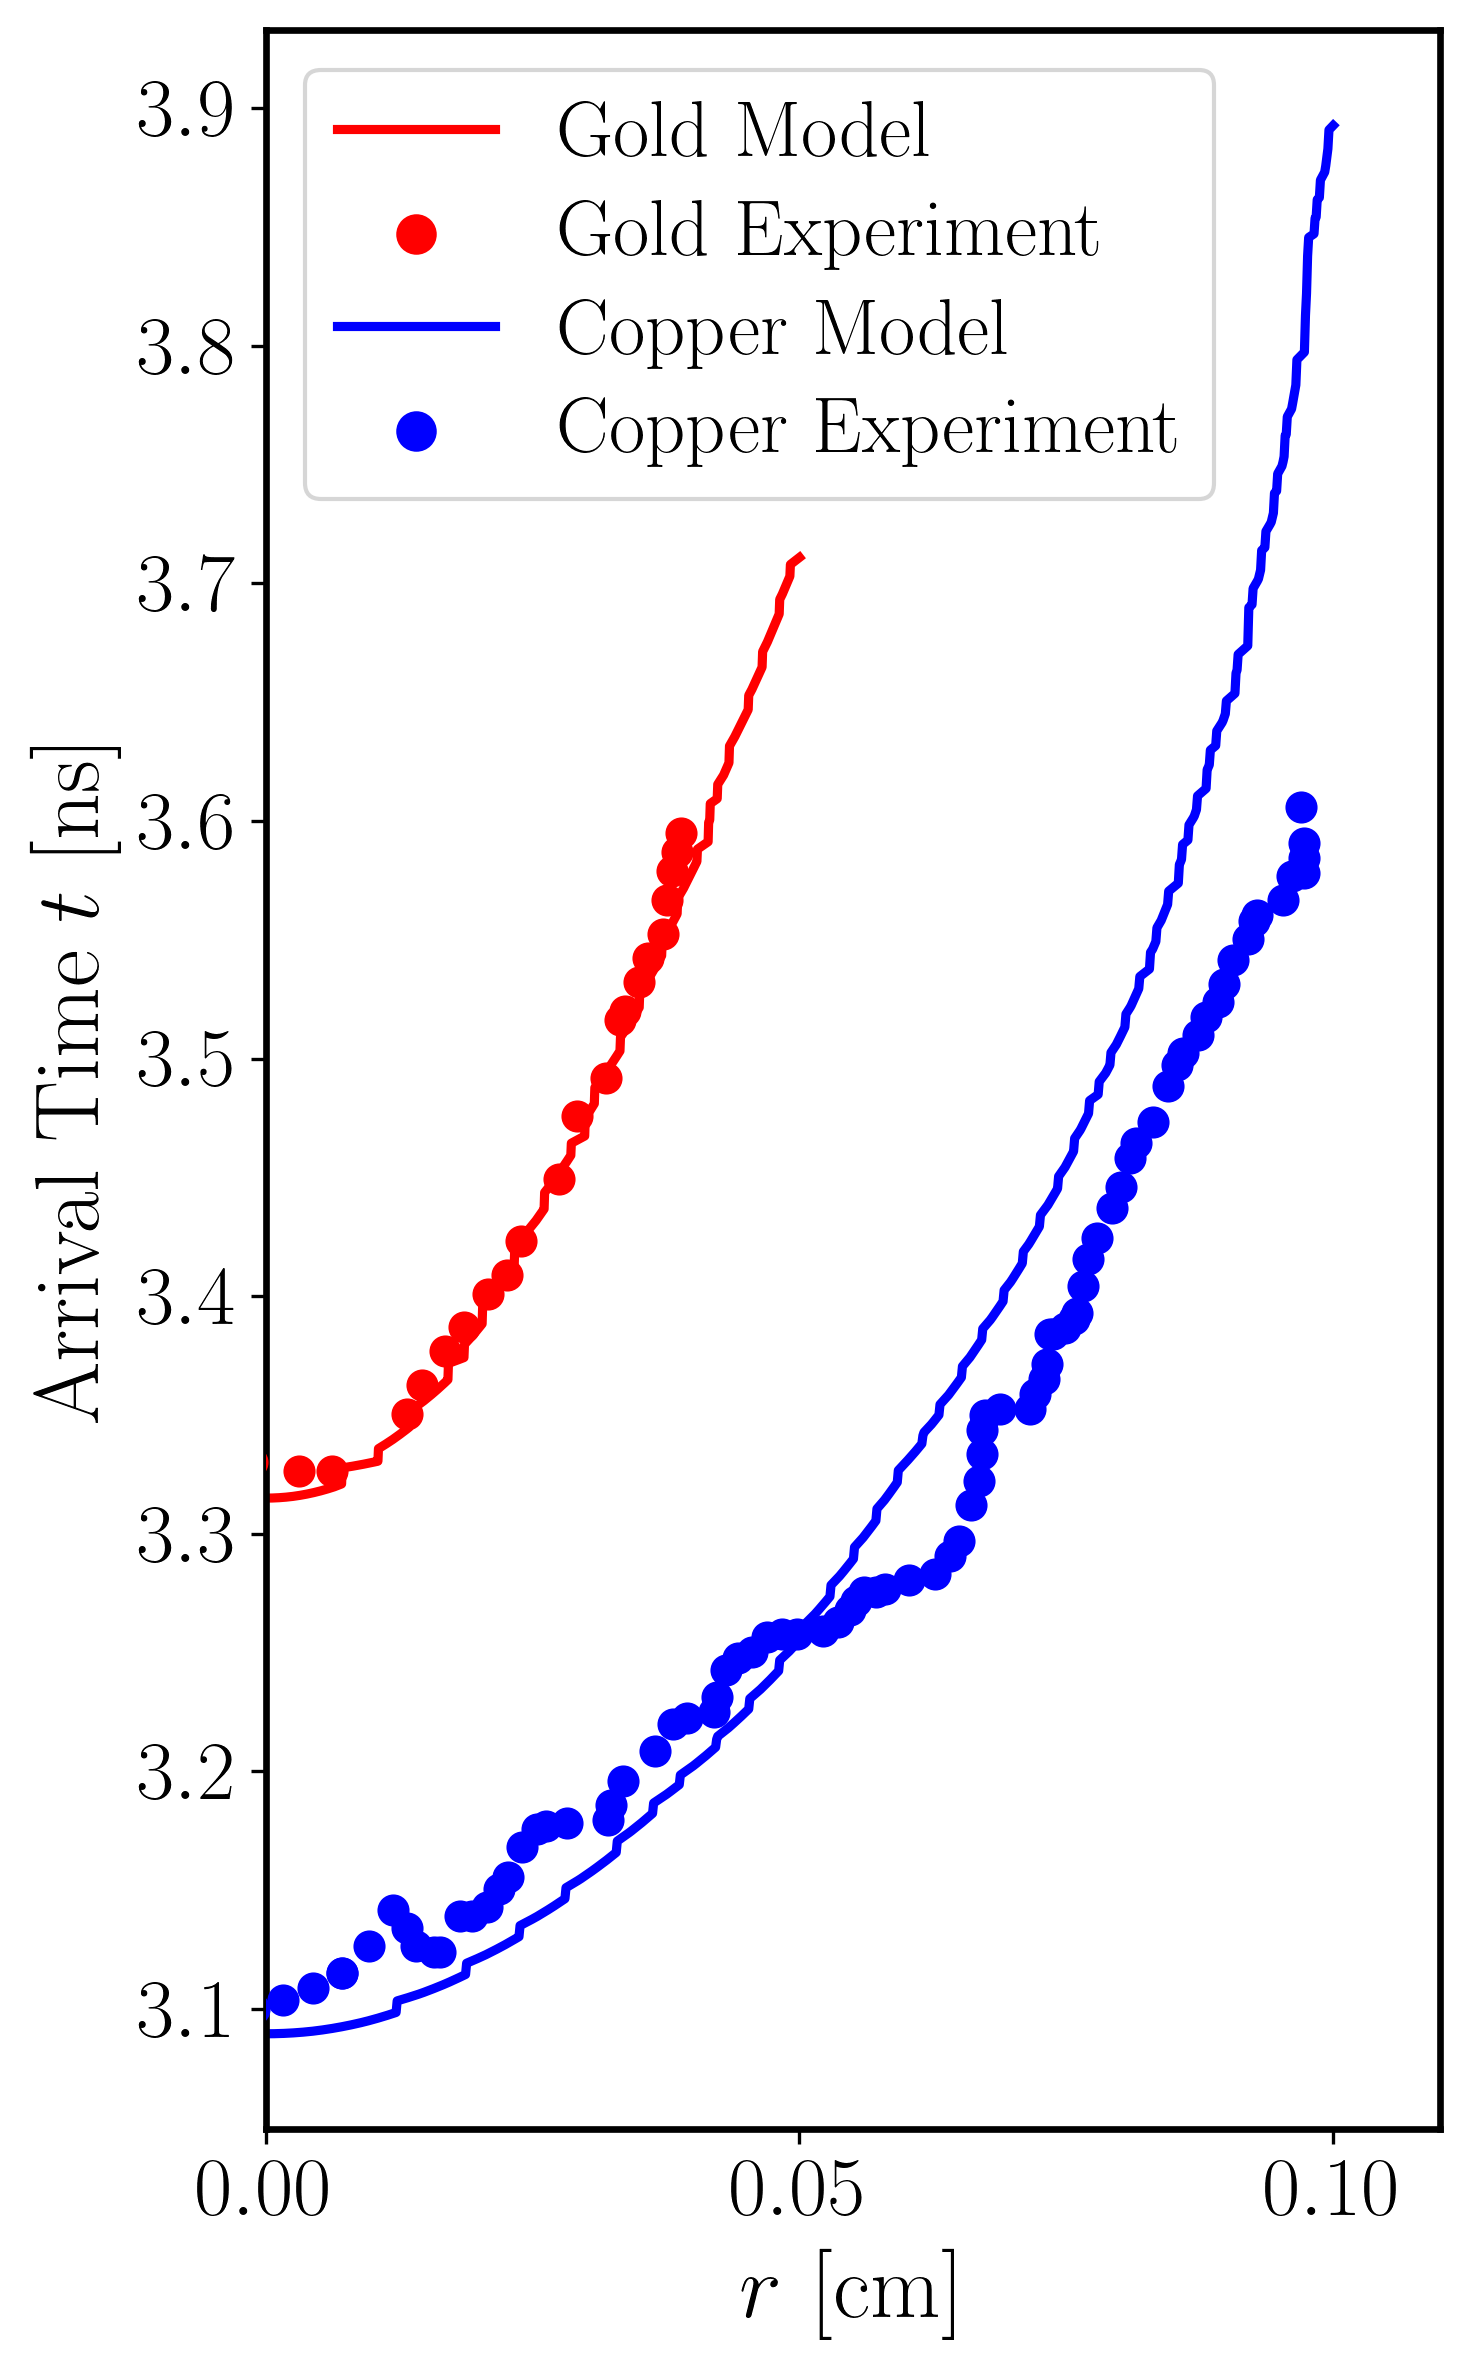
\includegraphics[width=\linewidth]{figures/french_expt.png}
        \vspace{-0.8em}
        \centerline{(c)}
    \end{minipage}
    \caption{(a) Model comparison with 2D diffusion simulation without hydrodynamics for the low-energy $\mathrm{SiO}_2$ case~\cite{Back2000PRL}, with Au coating, for 3 different times. (b) front curvature comparison with simulation between 4 different sleeves, Au, Cu, Be, and no sleeve (vacuum), showing the coating dependence. (c) Comparison with the French experiment of Courtois \textit{et al.}~\cite{Courtois2024}, measuring front-arrival time versus radius for Au (1.2 mm) and Cu (2 mm) coatings.}
    \label{fig:simulation_comparison}
\end{figure}

In addition, we compare the model curvature directly with experimental data from the French campaign~\cite{Courtois2024}, where front-arrival time is measured as a function of radius for Au- and Cu-coated tubes [Fig.~\ref{fig:simulation_comparison}(c)]. This comparison includes hydrodynamic effects, in particular wall ablation, which increase wall-energy absorption, lower the albedo, and therefore enhance the curvature. The effective mean-free-path correction is essential under these conditions because the Rosseland mean free path exceeds the tube diameter over much of the pulse. For Cu-coated foam, the maximum MFP is 1.5 mm versus a 2.0 mm tube diameter, so only a modest correction is required and best agreement is obtained with $n=2.5$. For Au-coated foam, the maximum MFP is 1.05 mm versus a 1.0 mm diameter, so the correction is substantially stronger and we use $n=1$. This trend suggests that larger diameter systems are less wall-loss dominated. Overall, the agreement shows that the model captures the dominant curvature physics under realistic experimental conditions. The MFP values are obtained from the optical depth across the heated region by integrating from $x=0$ to $0.9x_F(t)$ with the Henyey-like temperature distribution. The upper limit excludes the sharp front region, where the optical depth would otherwise become poorly behaved.

The front position alone describes the boundary of the heated region, but it does not specify how the deposited energy is distributed throughout the tube. To predict additional experimental observables, we therefore reconstruct the full two-dimensional temperature field behind the curved front. This provides $T(r,x,t)$ at every heated position and allows quantities such as the radial re-emission-flux profile, its curvature, and its evolution at a chosen time or diagnostic plane to be calculated directly from the model. We obtain this field by combining the corrected longitudinal temperature profile with the radial bessel function structure. The curved front determines which axial positions have been heated at each radius, while the temperature behind it follows the Henyey-like profile used in the one-dimensional solution~\cite{Hammer2003,Rosen2009}, with radial dependence entering through the local front position,
\begin{equation}\label{eq:henyey_profile}
T(r,x,t) = T_s(t)\left[1-\dfrac{x}{x_F(r,t)}\right]^{\frac{1}{4+\alpha-\beta}}
\end{equation}
where $x_F(r,t)$ is the curved heat-front position and $T_s(t)$ is the surface temperature obtained from the corrected 1D Marshak calculation. Evaluating this expression across the tube yields the full map of $T^4(r,x,t)$ shown in Fig.~\ref{fig:temperature_flux_curvature}(a), from which the observable re-emission pattern follows directly. At a diagnostic plane $x=x_{\mathrm{det}}$, the model flux is $\Phi(r,x_{\mathrm{det}},t)=\sigma_{\mathrm{SB}}T^4(r,x_{\mathrm{det}},t)$, and the resulting radial profile is normalized to its peak before comparison with the measured emission profile. Because wall losses cool the plasma near the tube boundary more strongly than near the axis, the edge temperature is lower, and the emitted flux there is correspondingly reduced, producing the depressed edge emission seen in Fig.~\ref{fig:temperature_flux_curvature}(b).

Figure~\ref{fig:temperature_flux_curvature}(c) shows an additional experimental curvature dataset from Back \textit{et al.}~\cite{Back2000POP} for Ta$_2$O$_5$, evaluated at the temporal peak of the emitted x-ray signal (0.5 ns after breakout). The samples are 0.25, 0.50, 0.75, and 1.00 mm long: the shorter samples (0.25 and 0.50 mm) are exposed to heating for a longer time, are therefore more diffusive, and are reproduced more accurately by the model. For the longer samples (0.75 and 1.00 mm), the diffusion approximation is less valid, and the agreement is correspondingly worse. This comparison highlights both the predictive strength and the validity limits of the diffusion-based model.

\begin{figure*}[t]
    \centering
    \begin{minipage}{0.38\textwidth}
        \centering
        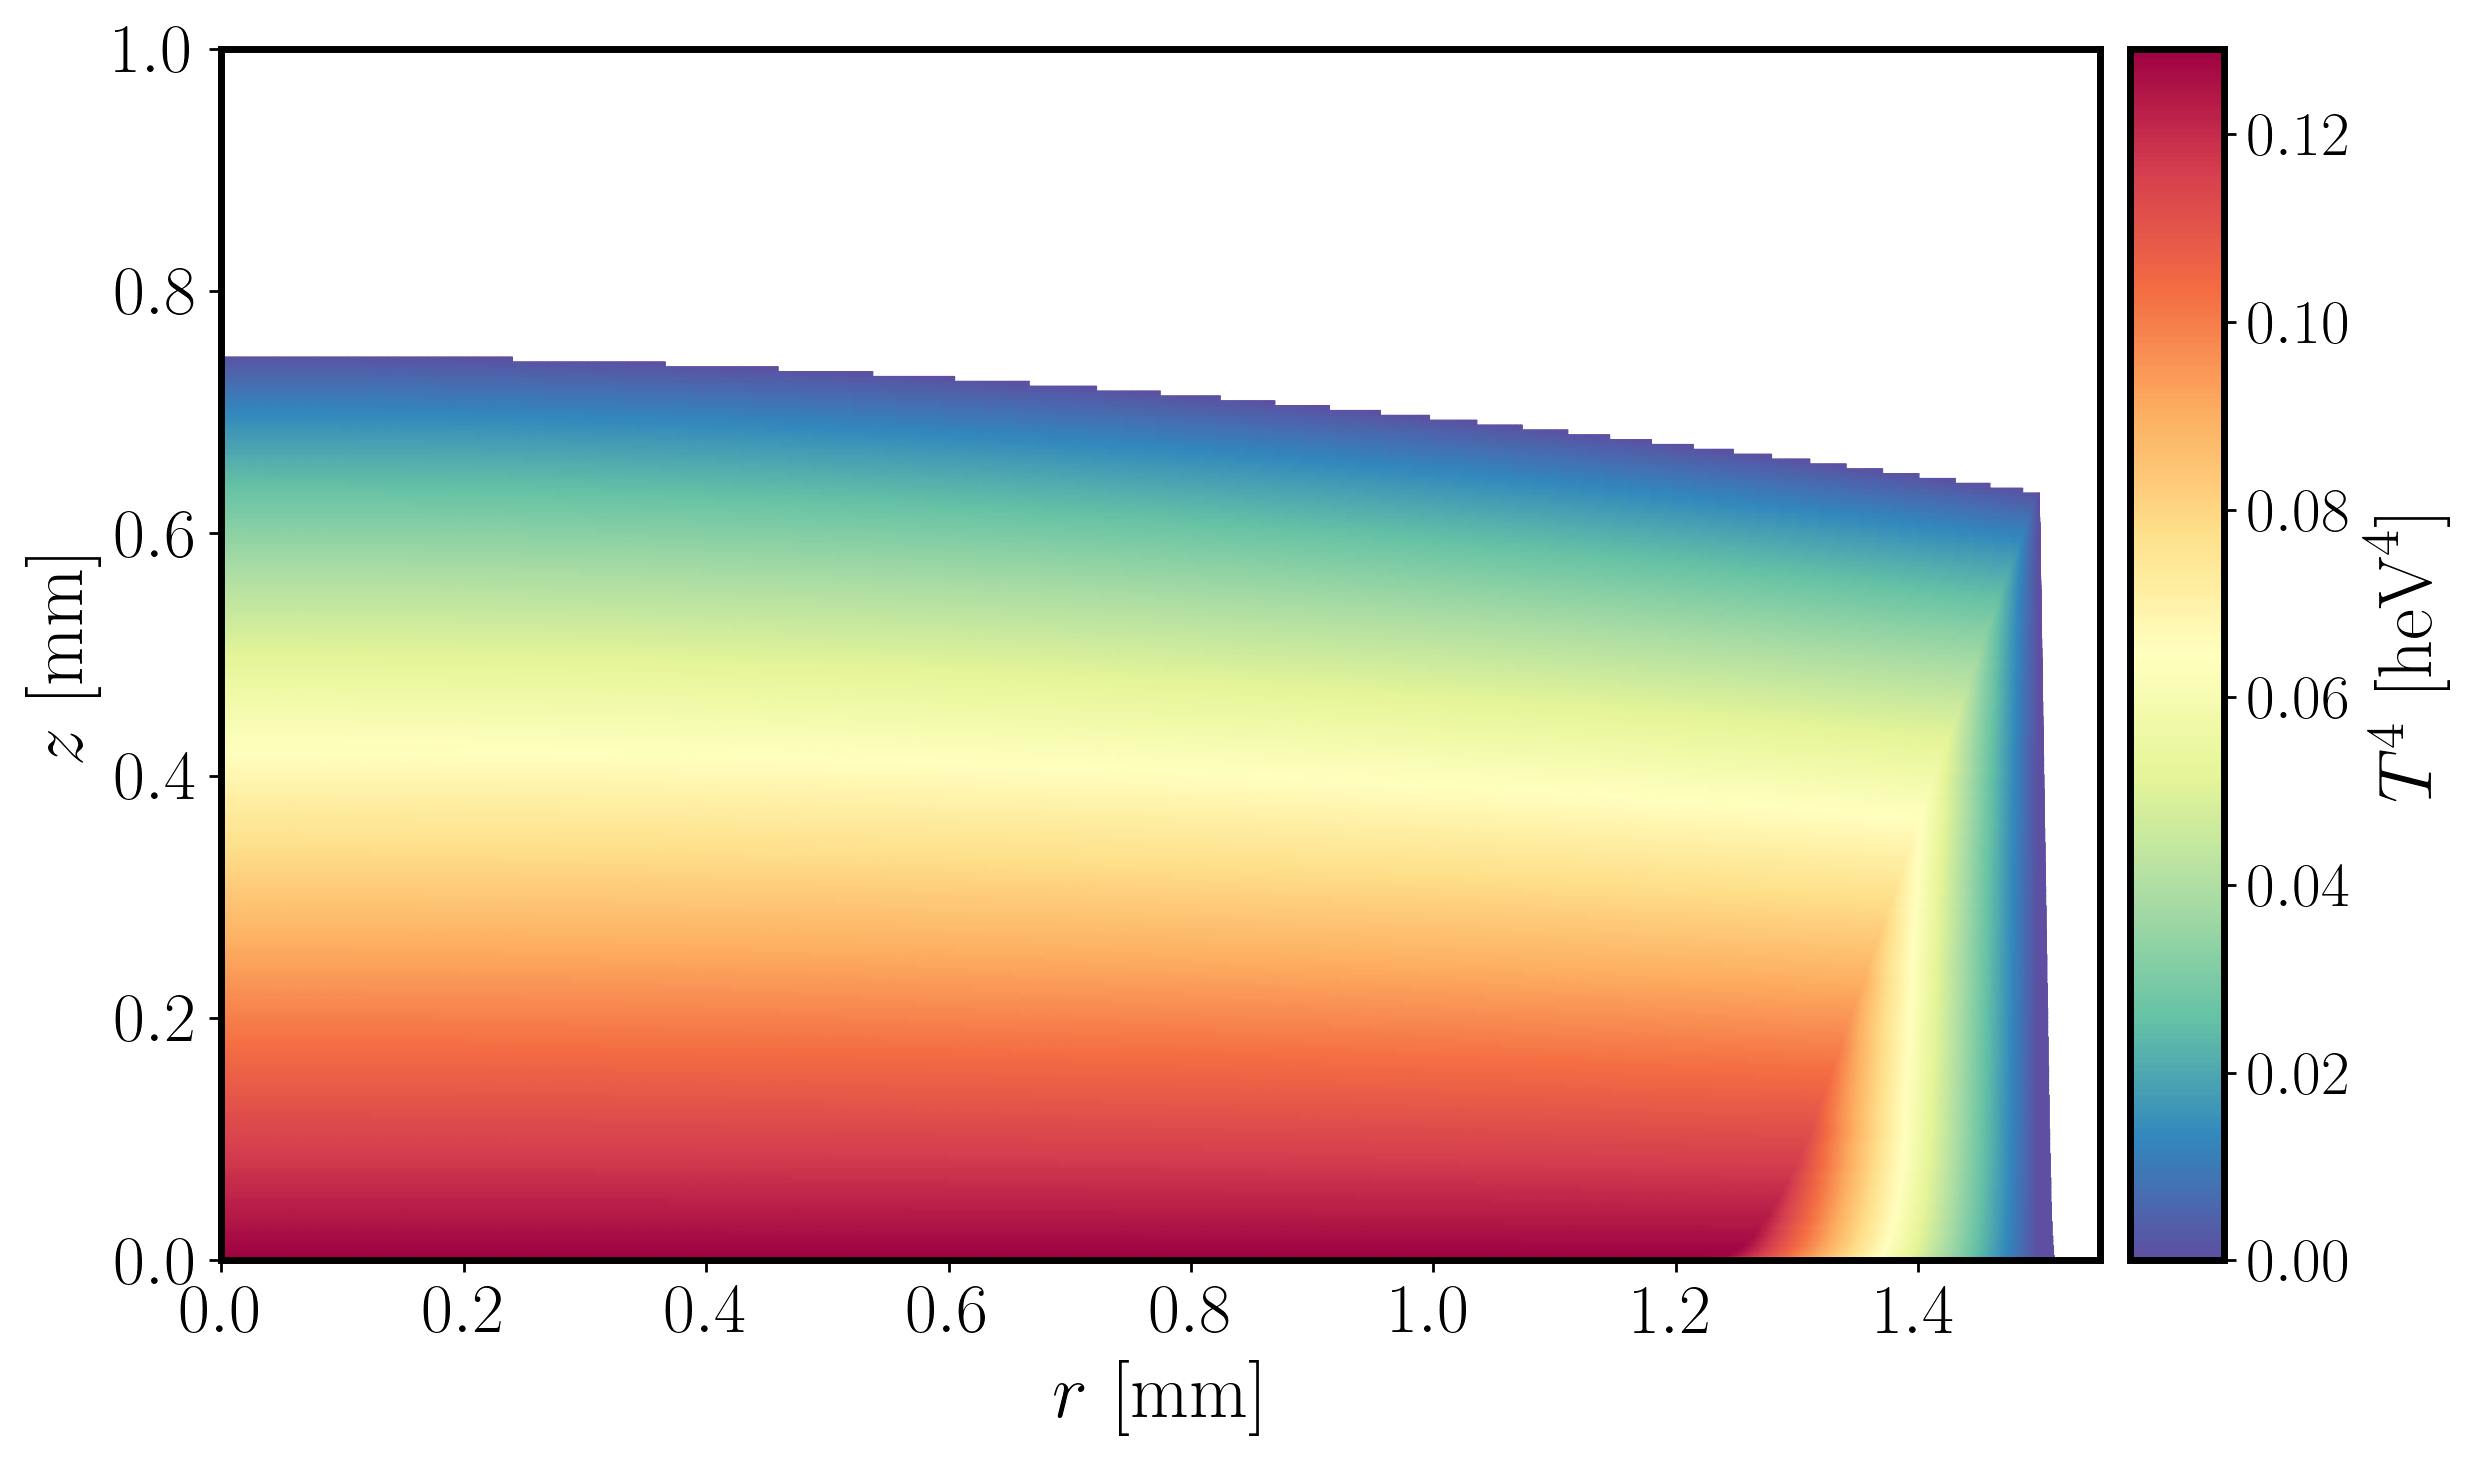
\includegraphics[width=\linewidth]{figures/prl_T4.png}
        \vspace{-0.8em}
        \centerline{(a)}
    \end{minipage}\hfill
    \begin{minipage}{0.26\textwidth}
        \centering
        
\includegraphics[width=\linewidth]{figures/back_prl_curve.png}
        \vspace{-0.8em}
        \centerline{(b)}
    \end{minipage}\hfill
    \begin{minipage}{0.3\textwidth}
        \centering
        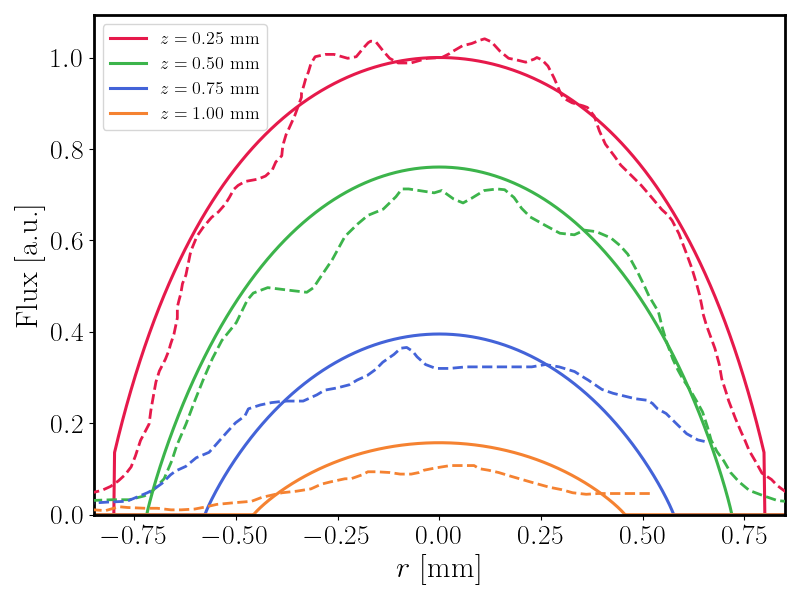
\includegraphics[width=\linewidth]{figures/back_pop_ta2o5_curve.png}
        \vspace{-0.8em}
        \centerline{(c)}
    \end{minipage}
    \caption{Temperature reconstruction and flux curvature. (a) Two-dimensional $T^4(r,z)$ profile obtained by the model at time 6 ns. (b) A cross section of the radial flux profile, compared with the Back \textit{et al.} radial intensity data, at 1mm inside the tube, 9.5 ns after the drive starts. (c) Additional experimental flux-curvature comparison for Ta$_2$O$_5$ from Back \textit{et al.}~\cite{Back2000POP}, taken at the temporal peak of the emitted x-ray signal (0.5 ns after breakout).}
    \label{fig:temperature_flux_curvature}
\end{figure*}

\begingroup
\setlength{\parskip}{0pt}
\setlength{\parindent}{1em}
% ============================================================================
%  V. CONCLUSION
% ============================================================================

We have developed a compact semi-analytic framework that connects the longitudinal evolution of a supersonic Marshak wave to its transverse structure and observable re-emission pattern in finite cylindrical targets. By combining the Marshak boundary closure with wall-energy loss, ablation-driven compression, finite-diameter transport, and a dynamic-albedo description of front curvature, the model identifies how each mechanism modifies propagation while retaining the speed and physical transparency of an analytic treatment. Comparisons with experiments and two-dimensional diffusion simulations show that this description captures the principal trends in front position, breakout, curvature, and sleeve-material dependence across a range of target configurations.

The remaining discrepancies also define the present limits of the framework. Its diffusion and LTE assumptions become less reliable when the heated region spans only a few optical depths, or when examining shorter times, while the reduced treatment of hydrodynamics cannot fully describe strongly evolving sleeve--foam interfaces. The model is therefore most useful as an interpretable predictive and diagnostic tool within the diffusive, supersonic regime, where it can isolate the mechanism limiting a particular experiment and guide choices of foam density, tube diameter, and temperature range.
\endgroup

% ============================================================================
%  REFERENCES
% ============================================================================
\begin{thebibliography}{99}

\bibitem{AbuShawareb2024}
H.~Abu-Shawareb \textit{et al.} (Indirect Drive ICF Collaboration),
Phys.\ Rev.\ Lett.\ \textbf{132}, 065102 (2024).

\bibitem{AbuShawareb2022}
H.~Abu-Shawareb \textit{et al.} (Indirect Drive ICF Collaboration),
Phys.\ Rev.\ Lett.\ \textbf{129}, 075001 (2022).

\bibitem{Lindl2004}
J.~D.~Lindl, P.~Amendt, R.~L.~Berger, S.~G.~Glendinning, and S.~H.~Glenzer,
Phys.\ Plasmas \textbf{11}, 339 (2004).

\bibitem{Hinkel2006PRL}
D.~E.~Hinkel, M.~B.~Schneider, B.~K.~Young, A.~B.~Langdon, E.~A.~Williams, M.~D.~Rosen, and L.~J.~Suter,
\textit{Creation of hot radiation environments in laser-driven targets},
Phys.\ Rev.\ Lett.\ \textbf{96}, 195001 (2006).

\bibitem{AfsharRad1994}
T.~Afshar-rad, M.~Desselberger, M.~Dunne, J.~Edwards, J.~M.~Foster, D.~Hoarty,
M.~W.~Jones, S.~J.~Rose, P.~A.~Rosen, R.~Taylor, and O.~Willi,
\textit{Supersonic Propagation of an Ionization Front in Low Density Foam Targets Driven by Thermal Radiation},
Phys.\ Rev.\ Lett.\ \textbf{73}, 74 (1994).

\bibitem{Massen1994}
J.~Massen, G.~D.~Tsakiris, K.~Eidmann, I.~B.~F\"oldes, Th.~L\"ower, R.~Sigel,
S.~Witkowski, H.~Nishimura, T.~Endo, H.~Shiraga, M.~Takagi, Y.~Kato, and S.~Nakai,
\textit{Supersonic radiative heat waves in low-density high-$Z$ material},
Phys.\ Rev.\ E \textbf{50}, 5130 (1994).

\bibitem{Back2000PRL}
C.~A.~Back, J.~D.~Bauer, J.~H.~Hammer \textit{et al.},
\textit{Diffusive, supersonic x-ray transport in radiatively heated foam cylinders},
Phys.\ Rev.\ Lett.\ \textbf{84}, 274 (2000).

\bibitem{Back2000POP}
C.~A.~Back, J.~D.~Bauer, O.~L.~Landen \textit{et al.},
\textit{Detailed measurements of a diffusive supersonic wave in a radiatively heated foam},
Phys.\ Plasmas \textbf{7}, 2126 (2000).

\bibitem{Moore2015}
A.~S.~Moore, T.~M.~Guymer, J.~Morton \textit{et al.},
\textit{Characterization of supersonic radiation diffusion waves},
J.\ Quant.\ Spectrosc.\ Radiat.\ Transfer \textbf{159}, 100 (2015).

\bibitem{Courtois2024}
C.~Courtois, R.~Gr\"oger, P.~Loiseau \textit{et al.},
\textit{Experimental measurements of supersonic radiation heat wave curvature in cylindrical tubes},
Phys.\ Plasmas \textbf{31}, 012707 (2024).

\bibitem{Keiter2008}
P.~Keiter, M.~Gunderson, J.~Foster \textit{et al.},
\textit{Radiation transport in inhomogeneous media},
Phys.\ Plasmas \textbf{15}, 056901 (2008).

\bibitem{Jiang2005}
S.~Jiang, Y.~Xu, Y.~Ding \textit{et al.},
\textit{Experimental investigation of supersonic radiation propagation in low-density plastic and copper-doped foams},
Sci.\ China Ser.\ G \textbf{48}, 549 (2005).

\bibitem{Zhang2010}
J.-Y.~Zhang, J.-M.~Yang, S.-E.~Jiang \textit{et al.},
\textit{Experimental observation of ionization and shock fronts in foam targets driven by thermal radiation},
Chin.\ Phys.\ B \textbf{19}, 025201 (2010).

\bibitem{Hammer2003}
J.~H.~Hammer and M.~D.~Rosen,
\textit{A consistent approach to solving the radiation diffusion equation},
Phys.\ Plasmas \textbf{10}, 1829 (2003).

\bibitem{Hurricane2006}
O.~A.~Hurricane and J.~H.~Hammer,
\textit{Bent Marshak waves},
Phys.\ Plasmas \textbf{13}, 113303 (2006).

\bibitem{Cohen2018}
A.~P.~Cohen and S.~I.~Heizler,
J.\ Comput.\ Theor.\ Transp.\ \textbf{47}, 378 (2018).

\bibitem{Cohen2020Key}
A.~P.~Cohen, G.~Malamud, and S.~I.~Heizler,
\textit{Key to understanding supersonic radiative Marshak waves using simple models and advanced simulations},
Phys.\ Rev.\ Research \textbf{2}, 023007 (2020).

\bibitem{Courtois2022}
C.~Courtois, R.~Gr\"oger, P.~Loiseau \textit{et al.},
\textit{Models for the propagation of radiation heat fronts in cylindrical tubes},
Phys.\ Plasmas \textbf{29}, 022704 (2022).

% \bibitem{Moore2012NIF}
% A.~S.~Moore, J.~L.~Kline, P.~A.~Keiter, J.~Morton, T.~M.~Guymer,
% G.~Magelssen, B.~Devolder, K.~A.~Mussack, R.~Peterson, J.~M.~Taccetti,
% N.~Lanier, M.~Stevenson, J.~Workman, K.~A.~Obrey, D.~Schmidt,
% C.~Hamilton, D.~Capelli, J.~Williams, B.~Randolph, F.~Fierro,
% J.~Martinez, B.~Patterson, N.~Bazin, and S.~Goodinga,
% \textit{NIF presentation} (2012).

\bibitem{Pomraning1979}
G.~C.~Pomraning,
\textit{The Equations of Radiation Hydrodynamics}
(Pergamon, Oxford, 1973).

\bibitem{Rosen2009}
M.~D.~Rosen,
\textit{Lectures in the Scottish Universities Summer School in Physics, 2005, on High Energy Laser Matter Interactions},
in \textit{High Energy Laser Matter Interactions}, edited by D.~A.~Jaroszynski, R.~Bingham, and R.~A.~Cairns
(CRC Press, Boca Raton, 2009), p.~325.

\bibitem{Olson2000}
G.~L.~Olson, L.~H.~Auer, and M.~L.~Hall,
\textit{Diffusion, $P_1$, and other approximate forms of radiation transport},
J.~Quant.~Spectrosc.~Radiat.~Transfer~\textbf{64}, 619 (2000).

\bibitem{ZeldovichRaizer2002}
B.~Ya.~Zel'dovich and P.~Yu.~Raizer,
\textit{Physics of Shock Waves and High-Temperature Hydrodynamic Phenomena}
(Dover, New York, 2002).

\bibitem{PakulaSigel1985}
R.~Pakula and R.~Sigel,
Phys.\ Fluids \textbf{28}, 232 (1985).

% \bibitem{Fleck1971}
% J.~A.~Fleck, Jr., and J.~D.~Cummings, Jr.,
% \textit{An implicit Monte Carlo scheme for calculating time and frequency dependent nonlinear radiation transport},
% J.~Comput.~Phys.~\textbf{8}, 313 (1971).

% \bibitem{Su1996}
% B.~Su and G.~L.~Olson,
% \textit{Benchmark results for the non-equilibrium Marshak diffusion problem},
% J.~Quant.~Spectrosc.~Radiat.~Transfer~\textbf{56}, 337 (1996).

\bibitem{Shussman2015}
T.~Shussman and S.~I.~Heizler,
\textit{Full self-similar solutions of the subsonic radiative heat equations},
Phys.\ Plasmas \textbf{22}, 082109 (2015).

\end{thebibliography}

\end{document}
